\documentclass{article}
\usepackage[margin=.5in, paperwidth=6in, paperheight=5in]{geometry}
\usepackage{ProofPower, graphicx, listings, alltt, enumerate}
\usepackage{animate}
\begin{document}
\section*{Specification}
This is a fighting game between two fighters, one controlled by the user and the other guided by probabilistic algorithms. The user is to press a key within timed intervals to have his/her fighter perform actions, while the computer utilizes a random number generator and weighted probabilities to have the other fighter perform actions. Actions are executed simultaneously.\\
There are three selectable fighter types: aggressive, balanced, and defensive. There are three attacks and three corresponding blocks: high, middle, and low. The aggressive fighter has more damage per attack but less defense per block, and has a higher chance of attacking than blocking when controlled by the program. The same idea applies to the defensive fighter.\\
Each action is implemented as a stance, with each stance having an attack quantity and a defense quantity. Damage is computed by subtracting the defender's stance's defense from the attacker's stance's attack.\\
The game continues until one fighter's health is depleted, upon which the controller of the other fighter is declared the victor.
\clearpage
\section*{Analysis}
\begin{alltt}
inputs:  mouse left click for menu navigation
         keyboard q, a, z for high, mid, low blocks
         keyboard w, s, x for high, mid, low attacks
process: have the player select a fighter type
         load initial images and user interface
         run animation
         every update:
             take user input to change fighter's stance
             run probabilistic algorithms to change other fighter's stance
             calculate damage taken and apply to healths
outputs: the score
         a boatload of fun!
\end{alltt}
\clearpage
\section*{Design} Algorithm:
Six Windows--created with FLUID/FLTK
\begin{itemize}
\item Background selection--User selects a background for the program to display
\begin{itemize}
\item make\_window()
\begin{itemize}
\item inputs: none
\item process: execution
\item output: creates a user-defined Fl\_Double\_Window
\end{itemize}
\item handle()
\begin{itemize}
\item inputs: mouse; (FL\_PUSH, FL\_DRAG)
\item processes: check if mouse is inside the selectionBox, if so, enable dragging the selectionBox
\item outputs: none
\end{itemize}
\item buttonPress()
\begin{itemize}
\item inputs: Fl\_Button press
\item processes: saves the user's selected background image in a global variable; hide current window using hide(); show main menu window with show()
\item outputs: main menu appears
\end{itemize}
\end{itemize}
\item Main menu--Three buttons, user can choose to start game, display info, or exit
\begin{itemize}
\item infoButtonPress()
\begin{itemize}
\item inputs: Fl\_Button press
\item processes: hide current window using hide(); show info window with show()
\item outputs: information window appears
\end{itemize}
\item startButtonPress()
\begin{itemize}
\item inputs: Fl\_Button press
\item processes: hide current window using hide(); show selection screen with show()
\item outputs: selection screen appears
\end{itemize}
\item quitButtonPress()
\begin{itemize}
\item inputs: Fl\_Button press
\item processes: close program with std::exit(0)
\item outputs: game ends
\end{itemize}
\end{itemize}
\item Information screen--Displays game and developer information in two text boxes
\begin{itemize}
\item returnButtonPress()
\begin{itemize}
\item inputs: Fl\_Button press
\item processes: hide current window using hide(); show main menu with show()
\item outputs: main menu appears
\end{itemize}
\end{itemize}
\item Selection Screen--User chooses one of three fighter types: Aggressive - has highest attack and lowest defense; Balanced - has balanced attack and defense statistics; Defensive - has highest defense and lowest attack
\begin{itemize}
\item buttonPress() -- one for each fighter type; fighter selection
\begin{itemize}
\item inputs: Fl\_Button press
\item processes: display corresponding Fighter image in a Box
\item outputs: image and text description of selected fighter appears
\end{itemize}
\item startButtonPress()
\begin{itemize}
\item inputs: Fl\_Button press
\item processes: initialize selected type of Fighter object; hide current window using hide(); show game window with show()
\item outputs: Fighter object created, game window appears
\end{itemize}
\end{itemize}
\item Game Screen--User plays the game, display two boxes (characters) for the computer and for the player. The user will press on appropriate keys to attack, defend, or do nothing -- each move will either cause the opponent damage or the user to take damage. Each character object has hitpoints and a score as a counter. The score is set at 100 -- as each turn progresses, the score decrements by one. When the score is depleted or one of the hitpoints is depleted, the game ends and the game screen closes.
\begin{itemize}
\item handle()
\begin{itemize}
\item inputs: keyboard presses (Q, A, Z, W, S, X, FL\_KEYBOARD, FL\_KEYPRESS) 
\item processes: store keyboard press in a char variable
\item output: image appears
\end{itemize}
\item runGame()
\begin{itemize}
\item inputs: refer to handle()
\item processes:
\begin{itemize}
\item render assigned image based on key stored from handle()
\item change player's Fighter's stance depending on specific key pressed
\item generate random number with rand() to randomly select opponent\PrOC{}\PrIA{}\PrJJ{}s move
\item process damage and adjust Fighters' health
\item decrement timer by one
\item check to see if either Fighter's health or the timer is zero
\item utilize Fl::repeat\_timeout() to use as a timed, repetitive function
\end{itemize}
\item outputs: image of appropriate attack and stance appears
\end{itemize}
\end{itemize}
\item End Screen--Displays "Game Over" along with health, score, and message reading "You Win!" or "You Lose"
\begin{itemize}
\item getScore()
\begin{itemize}
\item inputs: none
\item process: retrieve score and health. Display it. If neither score not health are 0, display "You Win" otherwise, "You Lose!"
\item outputs: display score, health, and game over message
\end{itemize}
\item buttonPress()
\begin{itemize}
\item inputs: Fl\_Button press
\item processes: hide() current window, show() Score Window
\item outputs: score window appears
\end{itemize}
\end{itemize}
\item Score Screen--
\begin{itemize}
\item doneButtonPress()
\begin{itemize}
\item inputs: Fl\_Button press
\item processes: hide current window, show main menu window
\item outputs: main menu appears
\end{itemize}
\item create fstream object and call fstream functions on it
\begin{itemize}
\item inputs: user enters a name
\item processes: read high scores from a file using <fstream> functions, called on fstream objects.
\begin{itemize}
\item fileObject.open()
\item isOpen(fileObject, lineString)
\item fileObject.close()
\end{itemize}
\item outputs: save high scores to the same file as before
\end{itemize}
\end{itemize}
\end{itemize}
\section*{Design (continued)}
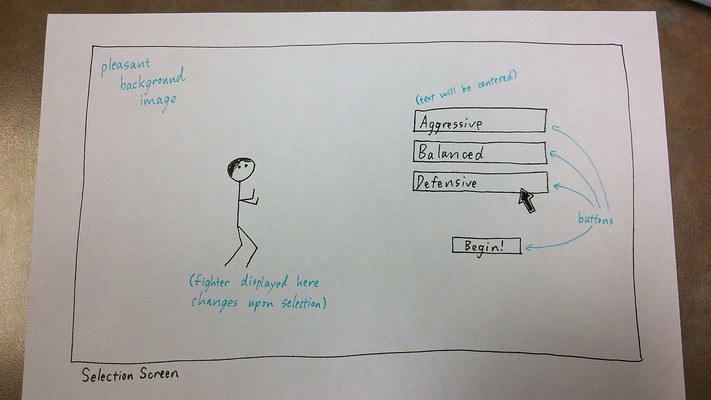
\includegraphics[scale=0.3]{design/selectionscreen.png}\\
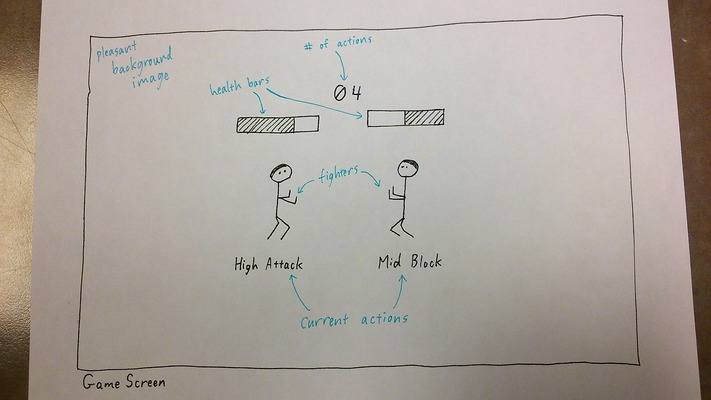
\includegraphics[scale=0.3]{design/gamescreen.png}
\section*{Implementation}
\begin{GFT}{C++ source code written to file fight.cpp}
\+\#include <iostream>\\
\+\#include <sstream>\\
\+\#include "fight.h"\\
\+\#include "Fighter.cpp"\\
\end{GFT}

\includegraphics[page=2]{Fighter.pdf}

\includegraphics[page=3]{Fighter.pdf}

\includegraphics[page=4]{Fighter.pdf}

\includegraphics[page=5]{Fighter.pdf}

\includegraphics[page=6]{Fighter.pdf}

\includegraphics[page=7]{Fighter.pdf}
\begin{GFT}{C++ source code appended to file fight.cpp}
\+\#include "backgroundselectionwindow.cpp"\\
\end{GFT}
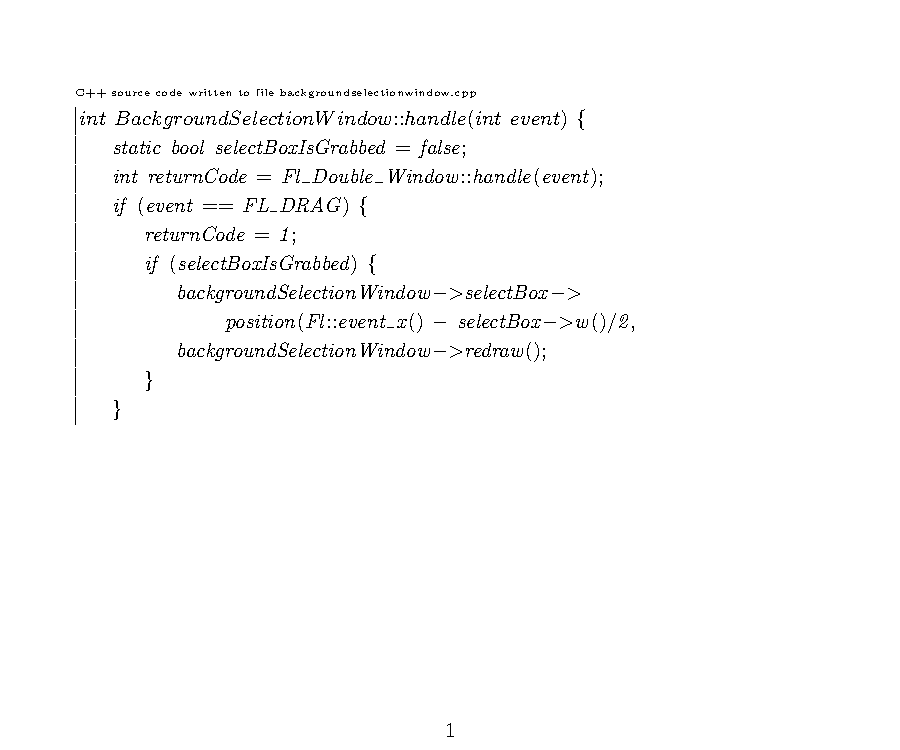
\includegraphics[page=1]{backgroundselectionwindow.pdf}
\includegraphics[page=2]{backgroundselectionwindow.pdf}
\includegraphics[page=3]{backgroundselectionwindow.pdf}
\includegraphics[page=4]{backgroundselectionwindow.pdf}
\begin{GFT}{C++ source code appended to file fight.cpp}
\+\#include "infowindow.cpp"\\
\end{GFT}
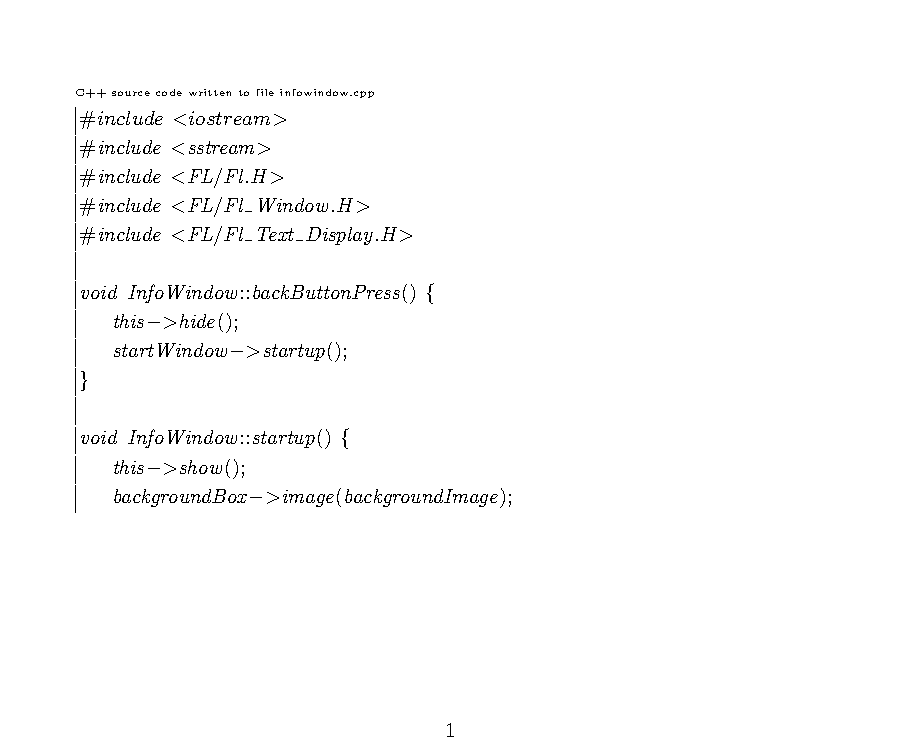
\includegraphics[page=1]{infowindow.pdf}
\includegraphics[page=2]{infowindow.pdf}
\begin{GFT}{C++ source code appended to file fight.cpp}
\+\#include "startwindow.cpp"\\
\end{GFT}

\begin{GFT}{C++ source code appended to file fight.cpp}
\+\#include "fighterselectionwindow.cpp"\\
\end{GFT}
\begin{GFT}{C++ source code appended to file fight.cpp}
\+\#include "gamewindow.cpp"\\
\end{GFT}
\begin{GFT}{C++ source code appended to file fight.cpp}
\+\#include "endwindow.cpp"\\
\end{GFT}
\begin{GFT}{C++ source code appended to file fight.cpp}
\+\#include "scorewindow.cpp"\\
\end{GFT}
\begin{GFT}{C++ source code appended to file fight.cpp}
\end{GFT}
Makes pointers to the objects created in Fluid on which to run the game on.
\begin{GFT}{C++ source code appended to file fight.cpp}
\+BackgroundSelectionWindow* backgroundSelectionWindow;\\
\+StartWindow* startWindow;\\
\+InfoWindow* infoWindow;\\
\+FighterSelectionWindow* fighterSelectionWindow;\\
\+GameWindow* gameWindow;\\
\+EndWindow* endWindow;\\
\+ScoreWindow* scoreWindow;\\
\+\\
\+Fl\_GIF\_Image* backgroundImage;\\
\+\\
\end{GFT}
Makes each window using functions defined in Fluid.
\begin{GFT}{C++ source code appended to file fight.cpp}
\+int main() \{\\
\+    backgroundSelectionWindow = makeBackgroundSelectionWindow();\\
\+    startWindow = makeStartWindow();\\
\+    infoWindow = makeInfoWindow();\\
\+    fighterSelectionWindow = makeFighterSelectionWindow();\\
\+    gameWindow = makeGameWindow();\\
\+    endWindow = makeEndWindow();\\
\+    scoreWindow = makeScoreWindow();\\
\+    backgroundSelectionWindow->show();\\
\+    return Fl::run();\\
\+\}\\
\end{GFT}
\section*{Implementation}
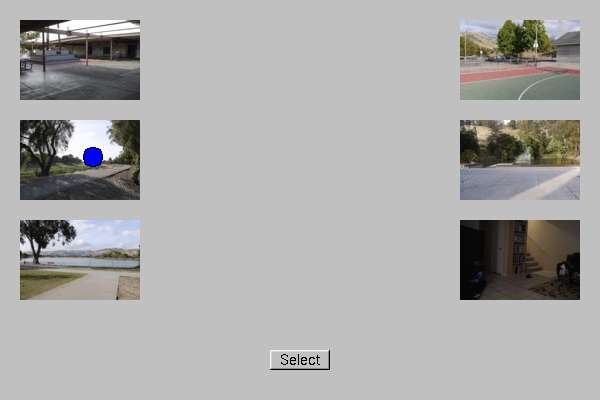
\includegraphics[scale=0.5]{test1.png}
\clearpage
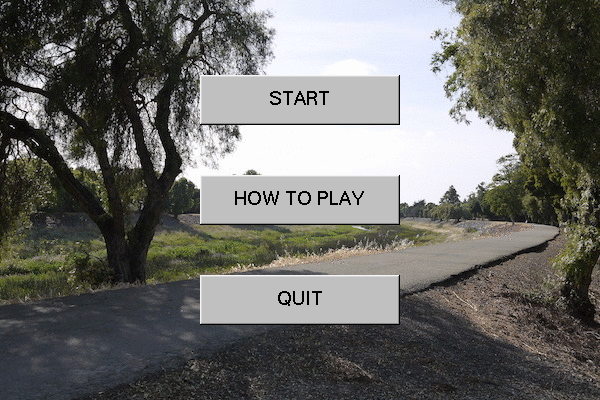
\includegraphics[scale=0.5]{test2.png}
\clearpage
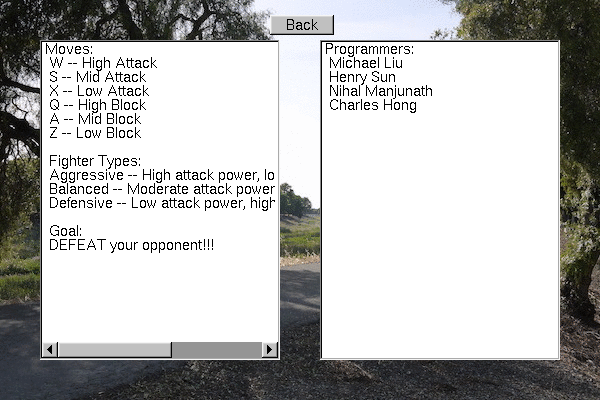
\includegraphics[scale=0.5]{test3.png}
\clearpage
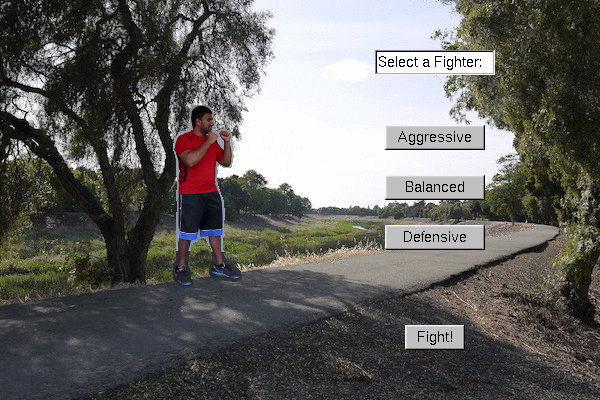
\includegraphics[scale=0.5]{test4.png}
\clearpage
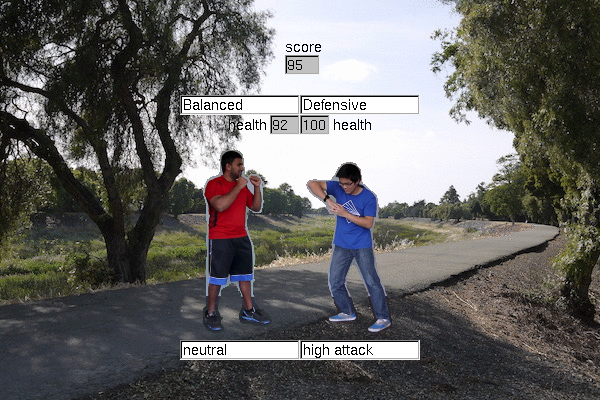
\includegraphics[scale=0.5]{test5.png}
\clearpage
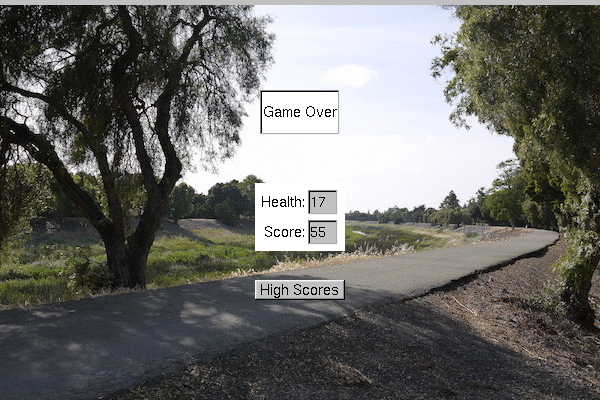
\includegraphics[scale=0.5]{test6.png}
\clearpage
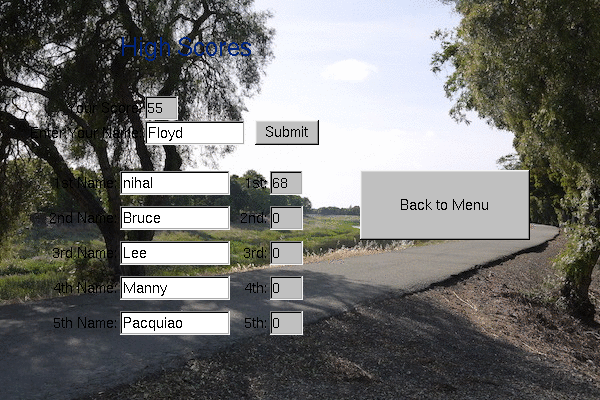
\includegraphics[scale=0.5]{test7.png}
%\section{GUI Code}
%\lstset{language=C++,breaklines=true}
%\lstinputlisting{fight.h}
%\lstinputlisting{fight.cxx}
\end{document}
